\section{Generalities}
An effort has been made to keep the same notations between the mathematical background and the \mudiff toolbox. A manual of every function is moreover provided by typing the classical \matlab command window 
\begin{lstlisting}
help name_of_the_function;
\end{lstlisting}

Because \mudiff includes all the integral operators that are needed in scattering (traces and normal derivative
traces of the single- and double-layer potentials), a large class of scattering problems can be solved. 
Concerning the geometrical configurations, any deterministic or random distribution of disks is possible. Finally,
\mudiff includes post-processing facilities like \eg: surface and far-fields computations, total and scattered exterior (near-field)
visualization\ldots

We now introduce the \mudiff  toolbox for Matlab by explaining the main predefined functions and their relations
with the previous mathematical derivations.
Section \ref{sec:PreProcessing}  shows how to define the scattering configuration (geometry and physical parameters). Section
 \ref{sec:ResolutionMuDiff}  presents the way the integral equations must be defined and solved.
  Finally, section \ref{sec:PostProcessing} describes the data post-processing. 

The \mudiff toolbox  is organized following the five subdirectories (see also figure \ref{fig:arbo} for a diagram of the arborescence):
\begin{itemize}
\item \texttt{mudiff/PreProcessing/}: pre-processing data functions (incident wave and geometry) (section \ref{sec:PreProcessing}).
\item \texttt{mudiff/IntOperators/}: functions for the four basic integral operators (dense and sparse structure)
used in the definition of the integral equations to solve (section \ref{sec:ResolutionMuDiff}). 
\item \texttt{mudiff/PostProcessing/}: post-processing functions of the solution (trace and normal derivative traces,
computation of the scattered/total wavefield 
at some points of the spatial domain or on a grid, far-field and RCS) 
(section \ref{sec:PostProcessing}).
\item \texttt{mudiff/Common/}: this directory includes functions that are used in \mudiff but which does not need to be known
from the standard user point of view.
\item \texttt{mudiff/Examples/}: various scripts are presented for the user in standard configurations.
\end{itemize}
In addition, the \mudiff user-guide, licence and credits can be found under the directory \texttt{mudiff/Doc/}.


\begin{figure}[p]
\tikzstyle{every node}=[draw=black,thick,anchor=west]
\begin{tikzpicture}[%
  grow via three points={one child at (0.5,-0.7) and
  two children at (0.5,-0.7) and (0.5,-1.4)},
  edge from parent path={(\tikzparentnode.south) |- (\tikzchildnode.west)}]
  \node {mu-diff/}
    child { node {Common}}
    child { node {Doc}}
    child { node {Examples}
      child { node {Benchmark}}
      child { node {TimeReversal}
      	  child { node {FarField}
      	    child { node {Common}}
      	    child { node {NonPenetrable}}
      	    child { node {Penetrable}}
      }
    }
    }
    child [missing] {}
    child [missing] {}
    child [missing] {}
    child [missing] {}
    child [missing] {}
    child [missing] {}
    child { node {IntOperators}
      child{node{Dense}
         child{node{Interface}
         child{node{Block}}
         child{node{Full}}
         }
      }
          child [missing] {}
    child [missing] {}
    child [missing] {}
      child{node{Sparse}
        child{node {Functions}}
         child{node{Interface}
           child{node{Block}}
           child{node{Full}}
         }
      }
    }
    child [missing] {}
    child [missing] {}
    child [missing] {}
    child [missing] {}
    child [missing] {}
    child [missing] {}
    child [missing] {}
    child [missing] {}
    child [missing] {}
    child { node {PostProcessing}
      child { node {FarField}
        child { node {Interface}}
       }
       child [missing] {}
      child { node {Geometry}}
      child { node {IncidentWave}}
      child { node {NearField}
        child { node {Functions}}
        child { node {Interface}}
       }
      }
    child [missing] {}
    child [missing] {}
    child [missing] {}
    child [missing] {}
    child [missing] {}
    child [missing] {}
    child [missing] {}
    child { node {Preprocessing}
        child { node {Fourier}}
        child { node {Geometry}}
        child { node {IncidentWave}
           child { node {Full}}
           child { node {Block}}
         }
	}
;
\end{tikzpicture}
\caption{Arborescence of \mudiff toolbox.}
\label{fig:arbo}
\end{figure}


\section{Common argument and notations}

A large number of arguments of the \mudiff functions are the same. For the sake of conciseness and if nothing is specified, the following arguments refer to the below ones, where the indices $p$ and $q$ vary from $1$ to $M$ (or \code{N\_scat} in the \mudiff language). In addition, every function or value specific to \mudiff are written with this \code{font}. 

\paragraph{Geometry:}

\begin{center}
%\rowcolors{1}{white}{gray}
\begin{tabular}{|c |c | p{10cm}|}
\hline Name & Size & Content\\[0.2cm]\hline\hline
\tabcode{N\_scat} & $[1\times 1]$ & Number of obstacles $M$.\\\hline
\tabcode{O} & $[2\times \Nscat]$ & Matrix of the centers of the disks such that \code{O(1,p)} (resp. \code{O(2,p)}) is the $x-$coordinate (resp. $y-$coordinate) of the $p^{th}$ obstacle.\\\hline
\tabcode{Op} & $[2\times 1]$ & Coordinates of the $p^{th}$ scatterer.\\\hline
\tabcode{Oq} & $[2\times 1]$ & Coordinates of the $q^{th}$ scatterer.\\\hline
\tabcode{a} & $[1\times \Nscat]$ & Vector of the radii of the disks such that \code{a(p)} is the radius of the $p^{th}$ scatterer.\\\hline
\tabcode{ap} & $[1\times 1]$ & Radius of the $p^{th}$ scatterer.\\\hline
\tabcode{aq} & $[1\times 1]$ & Radius of the $q^{th}$ scatterer.\\\hline
\end{tabular}
\end{center}

\paragraph{Parameters (wavenumbers, incident waves, fourier series, \ldots):}
\begin{center}
\begin{tabular}{|c |c | p{10cm}|}
\hline Name & Size & Content\\[0.2cm]\hline\hline
\tabcode{beta\_inc} & $[1\times 1]$ & Angle of direction $\beta$ of a plane wave $e^{ik (\cos(\beta)x + \sin(\beta)y)}$.\\\hline
\tabcode{XS} & $[2\times 1]$ & Center $(x_s,y_s)$ of a point source: $x_s=$\code{XS(1)} and $y_s=$\code{XS(2)}. A point source wave is given by $i/4\Hz(k\|\xx-\xx_s\|)$, with $\xx=(x,y)$ and $\xx_s=(x_s,y_s)$ and $\Hz$ the zeroth order Hankel function of first kind.\\\hline
\tabcode{k} & $[1\times 1]$ & Wavenumber $k$ in the vacuum.\\\hline
\tabcode{k\_int} & $[1\times \Nscat]$ & Wavenumbers in the obstacles: $\kintp=$\code{k\_int(p)}. If \code{k\_int} is a scalar then $\kintp$ = \code{k\_int} for all $p$.\\\hline
\tabcode{M\_modes} & $[1\times \Nscat]$ & Vector of index of truncation of the Fourier series, \ie \code{M\_modes(p)}=$\Np$\\\hline
\tabcode{Np} & $[1\times 1]$ & Corresponds to $\Np$, the truncation index in the Fourier serie.\\\hline
\tabcode{Nq} & $[1\times 1]$ & Corresponds to $\Nq$, the truncation index in the Fourier serie.\\\hline
\end{tabular}
\end{center}

\paragraph{Integral operators:} as explained in Section \ref{??}, they are indexed and named by the following table:
\begin{center}
\begin{tabular}{|c |c | c | p{9cm}|}
\hline Index & Letter & \mudiff abreviation & Operator \\\hline\hline
0 & - & - & Null operator \\[0.2cm]\hline
1 & $I$ & \tabcode{Identity} & Identity\\[0.2cm]\hline
2 & $L$ & \tabcode{SingleLayer} & $\dsp L\rho = \int_{\Gamma}G(\xx,\yy)\rho(\yy)\;\dd\yy$\\[0.2cm]\hline
3 & $M$ & \tabcode{DoubleLayer} & $\dsp M\lambda = -\int_{\Gamma}\dny G(\xx,\yy)\lambda(\yy)\;\dd\yy$\\[0.2cm]\hline
4 & $N$  & \tabcode{DnSingleLayer}& $\dsp N\rho = \dnx\int_{\Gamma}G(\xx,\yy)\rho(\yy)\;\dd\yy$\\[0.2cm]\hline
5 & $D$  & \tabcode{DnDoubleLayer}&$\dsp D\lambda = -\dnx\int_{\Gamma}\dny G(\xx,\yy)\lambda(\yy)\;\dd\yy$\\[0.2cm] \hline
6 & $\hat{L}L$  & \tabcode{PrecondDirichlet}& Single-scattering preconditioned trace of the single-layer operator (see (\S\ref{sec:SingleScat}))\\[0.2cm]\hline
7 & $\hat{D}D$  & \tabcode{PrecondNeumann}& Single-scattering preconditioned normal derivative trace of the double-layer operator (see (\S\ref{sec:SingleScat}))\\ \hline
\end{tabular}
\end{center}


\section{Pre-Processing}\label{sec:PreProcessing}

The pre-processing in \mudiff consists in defining the right-hand side (or the incident wave) and the geometry (the obstacles). The associated functions are located respectively in the folder \folder{mudiff/PreProcessing/IncidentWave} and in \folder{mudiff/PreProcessing/Geometry}.

\subsection{Geometry: creating the obstacles}

The obstacles are stored in memory as a row vector \code{a} containing the radii of the disks and a [$2\times\code{N\_scat}$] matrix \code{O} containing the centers of the disks (\code{O(1,p}=$x-$ and \code{O(2,p}=$y-$ coordinates of the center of the $p^{th}$ disk). These two arrays can be created either manually or using some built in functions.

\subsubsection{Manually}

The disks can be created manually by simply creating the two variables \code{O} and \code{a} containing respectively the coordinates of the disks and their radii. For example, for three obstacles placed on $(-1,2)$, $(5,5)$ and $(-15,10)$ with radii $0.1$, $0.5$ and $10$:
\begin{lstlisting}
O = [-1, 5, 2 ; -15, 5, 10];
a = [0.1, 0.5, 10];
\end{lstlisting}

\subsubsection{Periodic placement}
\label{secFun:RectangularLattice}
\label{secFun:TriangularLattice}

Two build-in functions are available with the toolbox to create disks periodically, with a rectangular or a triangular lattice, as shown on figure \ref{fig:lattices}. The two functions must be called as follows, first for the rectangular lattice:
\begin{lstlisting}
O = RectangularLattice(bx, by, Nx, Ny, OPTIONS);
\end{lstlisting}
and second for the triangular lattice:
\begin{lstlisting}
O = TriangularLattice(bx, by, Nx, Ny, OPTIONS);
\end{lstlisting}
where the arguments are:
\begin{itemize}
\item \code{bx}: distance separating two centers in the $x-$ direction (be careful with the radii of the disks to avoid overlapping!).
\item \code{by}: distance separating two row of obstacles in the $y-$ direction.
\item \code{Nx}: number of disks in a row.
\item \code{Ny}: number of rows.
\end{itemize}
For both functions, the vector of radii must be built separately and manually. For a set of unitary disks, the following command does the work:
\begin{lstlisting}
a = ones(size(O,2));
\end{lstlisting}

The available options are (same for \RectangularLattice and \TriangularLattice):
\begin{itemize}
\item \code{RectangularLattice(..., 'Center', Ostart)}
Place the first disk on Ostart position, Ostart being a [2x1] vector. (Default: $[0;0]$).
 \item \code{RectangularLattice(..., 'Direction', DIR)}
Pace the row in the increasing y-direction (DIR=+1) or decreasing y-diretion (DIR=-1). Default: DIR+1.
\end{itemize}

\paragraph{Example:} Building a rectangle of $3$ unit disks and $4$ rows. Each disks is separated from a distance of $1.5$ (so the centers from a distance of $3.5$):
\begin{lstlisting}
O = RectangularLattice(3.5, 3.5, 3, 4);
a = ones(size(O,2));
\end{lstlisting}

\begin{figure}
\centering
\subfigure[Rectangular lattice]{\begin{tikzpicture}
 \pgftext{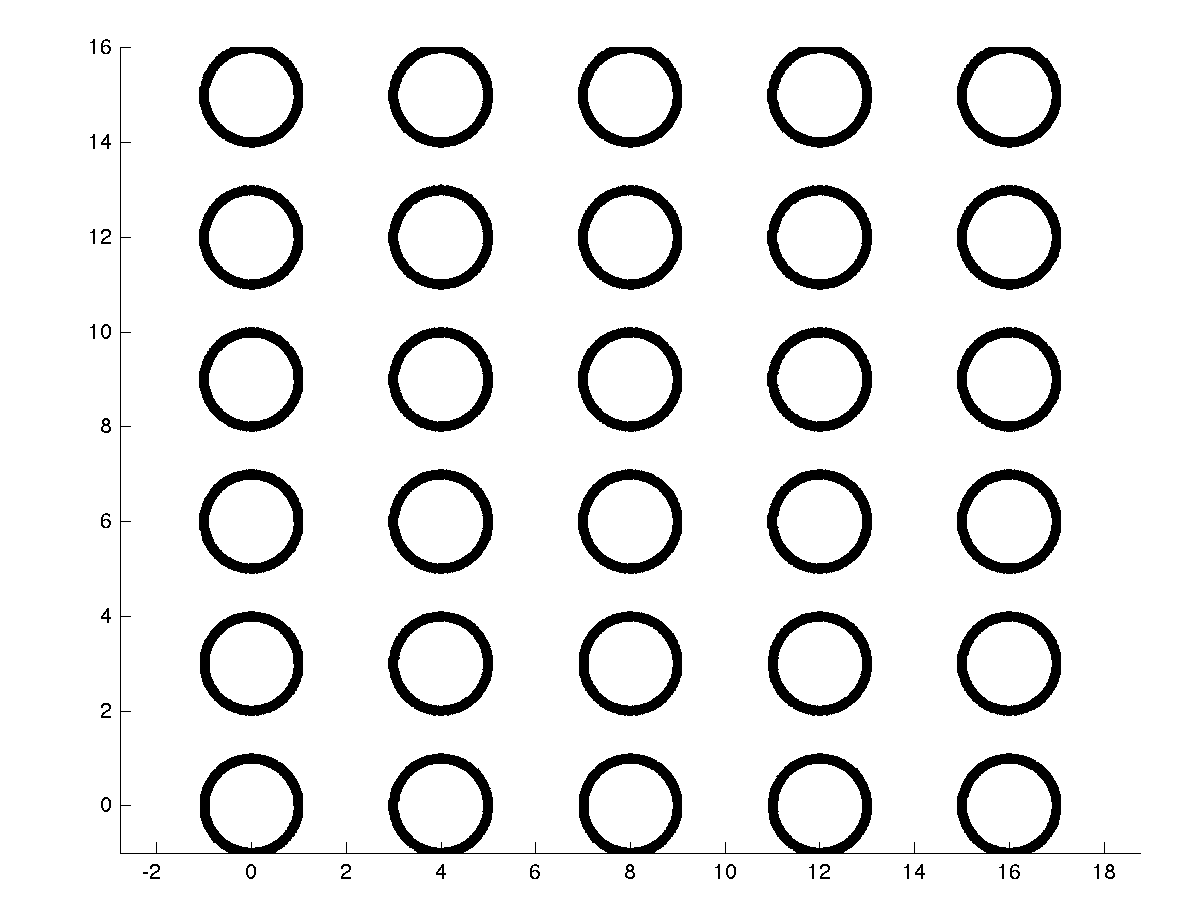
\includegraphics[width=0.45\textwidth]{./img/obstacles/rectangular.png}}
 \draw (10pt,-75pt) node[below]{\footnotesize $x_{1}$} ;
 \draw (-92pt,10pt) node[below]{\footnotesize $x_{2}$} ;
\end{tikzpicture}}\quad\subfigure[Triangular lattice]{\begin{tikzpicture}
 \pgftext{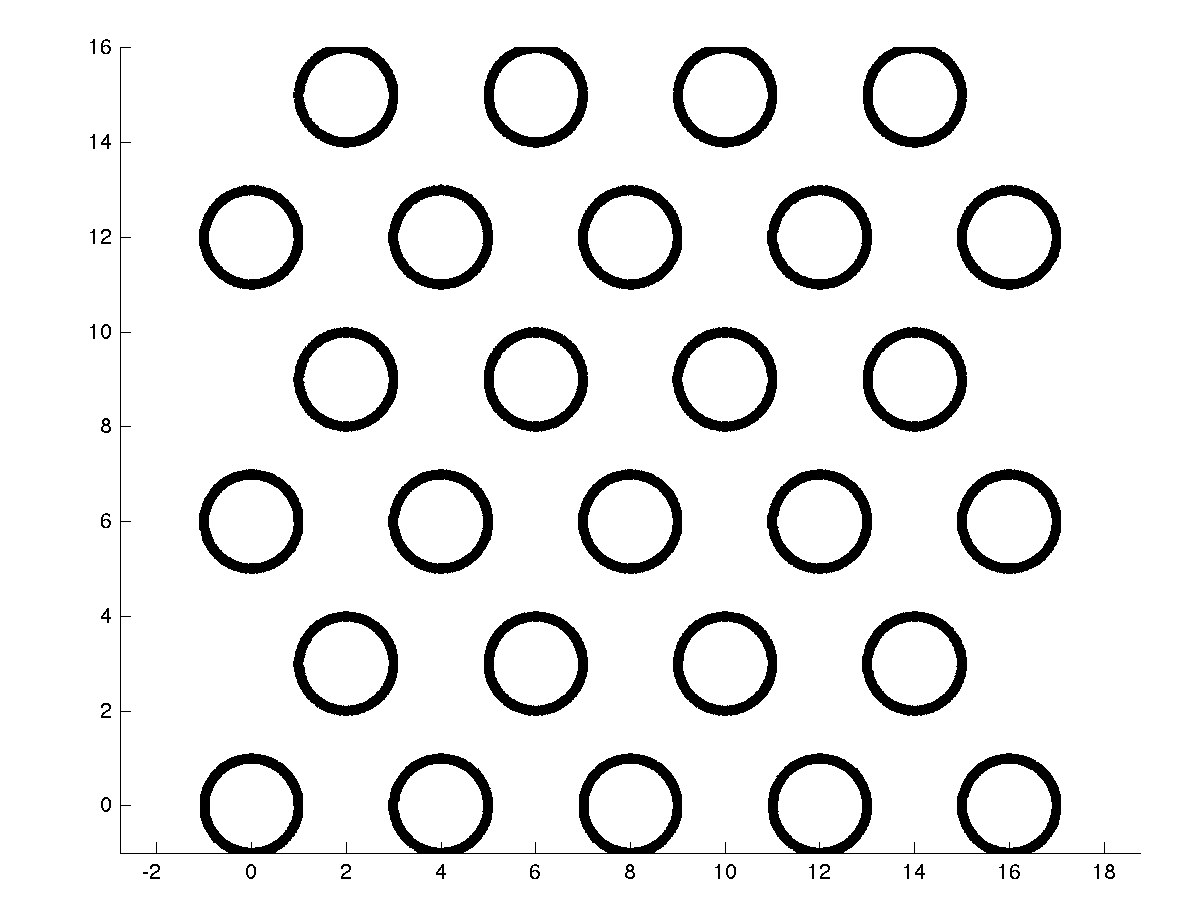
\includegraphics[width=0.45\textwidth]{./img/obstacles/triangular.png}}
 \draw (10pt,-75pt) node[below]{\footnotesize $x_{1}$} ;
 \draw (-92pt,10pt) node[below]{\footnotesize $x_{2}$} ;
\end{tikzpicture}}
\caption{Rectangular (left) and triangular (right) lattice with \code{bx}=3, \code{by}=4, \code{Nx} = 5, \code{Ny}=6.}
\label{fig:lattices}
\end{figure}


\subsubsection{Random placement}
\label{secFun:CreateRandomDisks}

\mudiff provides a function \CreateRandomDisks to randomly place \code{N\_scat} obstacles in a box $[\code{xmin}, \code{xmax}]\times[\code{ymin},\code{ymax}]$ with also a random radius. In its simplest version, the function is called as:
\begin{lstlisting}
[O, a] = CreateRandomDisks(xmin, xmax, ymin, ymax, N_scat);
\end{lstlisting}
In that case, \CreateRandomDisks builds \code{N\_scat} disk with unit radius in the desired box. The function takes care to not overlap the disks. Note that it is possible that the function does not succeed to place the obstacle (\eg if the user asks for too many obstacles in a small box) and hence a security has been set: only $500$ trials are allowed per disk. 

The function comes along with a large set of optional arguments:
\begin{lstlisting}
[O, a] = CreateRandomDisks(xmin, xmax, ymin, ymax, N_scat, 
           amin, amax, dmim, dmax, O_avoid, a_avoid, dmin_avoid, dmax_avoid);
\end{lstlisting}
where every additional arguments is optional (but the order must be kept (\code{amin} must be set, then \code{amax}, etc.!) and given by:
\begin{center}
\begin{tabular}{|c |c|c | p{10cm}|}
\hline Variable & Type & Default & Action\\\hline
\tabcode{amin} & scalar  & 1 & Minimal (random) radius of the obstacles allowed \\\hline
\tabcode{amax} & scalar  & 1 & Maximal (random) radius of the obstacles  allowed\\\hline
\tabcode{dmin} & scalar & \tabcode{realmin} & Minimal distance allowed between two obstacle (not between the centers!). Setting $\leq 0$  value will set \code{dmin} to \code{realmin} (\ie ignore it)\\\hline
\tabcode{dmax} & scalar & \tabcode{realmax} & Maximal distance allowed between two obstacle (not between the centers!). The maximal distance is quickly reached! Setting $\leq 0$  value will set \code{dmax} to \code{realmax} (\ie ignore it).\\\hline
\tabcode{O\_avoid} & $[2 \times N]$ & \tabcode{[]} & Center of \code{N} hole(s) where the obstacles must not overlap. Usefull for example for point source location.\\\hline
\tabcode{a\_avoid} & $[1 \times N]$ & \tabcode{[]} & Radii of the \code{N} holes\\\hline
\tabcode{dmin\_avoid} & $[1 \times N]$ & \tabcode{[]} & Minimal distance between an obstacle and a hole\\\hline
\end{tabular}
\end{center}
The ``holes'', represented by the \code{*\_avoid} arguments, are disks where the obstacles must not overlap, for example where a point source is emitting a wave. 

\paragraph{Example 1:} creating \code{N\_scat} random disks with random radii:
\begin{lstlisting}
[O, a] = CreateRandomDisks(xmin, xmax, ymin, ymax, N_scat, amin, amax);
\end{lstlisting}
\paragraph{Example 2:} building 7 obstacles in the box $[-10,10]\times[-10,10]$ with radii between $0.1$ and $0.5$. The disks must be separated at minimum by a distance of $0.1$ and without maximum value. The command is then:
\begin{lstlisting}
[O, a] = CreateRandomDisks(-10, 10, -10, 10, 7, 0.1, 0.5, 0.1, -1);
\end{lstlisting}
\paragraph{Example 3:} now imagine that a point source is located on $(2,2)$ and that the obstacles must be separated from the source from at least a distance of $0.3$, then the ``\code{*\_avoid}'' arguments can be used and command can be
\begin{lstlisting}
[O, a] = CreateRandomDisks(-10, 10, -10, 10, 7, 0.1, 0.5, 0.1, -1, [2;2], 0.3);
\end{lstlisting}
The disk centered on $(2,2)$ with radius $0.3$ will then be avoided. A second option is to set \code{a\_void} to zero and set the minimal distance \code{dmin\_avoid} to $0.3$:
\begin{lstlisting}
[O, a] = CreateRandomDisks(-10, 10, -10, 10, 7, 0.1, 0.5, 0.1, -1, [2;2], 0, 0.3);
\end{lstlisting}


\begin{remark}
\label{secFun:CheckPlacement}
To verify if a disk is well placed, \CreateRandomDisks calls \CheckPlacement function, which can also be useful for a user who is placing the obstacles manually.
\end{remark}

\subsubsection{Removing disks}
\label{secFun:RemoveDisk}

The function \RemoveDisk aims to remove some disks of the geometrical configuration, either disk by disk, by row or by column or by radius. This can be useful for example to delete a row of disks. Here is its syntax
\begin{lstlisting}
[O,a] = RemoveDisk(O_old, a_old, ...);
\end{lstlisting}
where \code{O\_old} and \code{a\_old} are the centers and radii of the current geometry. Without optional argument, the function has no effect. The available arguments are:
\begin{itemize}
\item \code{[O,a] = RemoveDisk(..., 'X', [X1, X2, .., XN]);}\\
Remove all the disks which center has its $x-$abscissa equal to \code{X1}, \code{X2}, \ldots, or \code{XN}
\item \code{[O,a] = RemoveDisk(...,  'Y', [Y1, Y2, ..., YN]);}\\
Remove all the disks which center has its $y$-ordinate \code{Y1}, \code{Y2}, \ldots, or \code{YN}
\item \code{[O,a] = RemoveDisk(..., 'XY', [[X1;Y1], [X2;Y2], ..., [XN;YN]]);}\\
Remove all the disks which center has for coordinates \code{[X1;Y1]}, \code{[X2;Y2]}, \ldots, or \code{[XN;YN]}
\item \code{[O,a] = RemoveDisk(..., 'Radius', [a1, a2, ..., aN]);}\\
Remove all the disk which radius is equal to \code{a1}, \code{a2}, \ldots, or \code{aN}
\item \code{[O,a] = RemoveDisk(..., 'Verbosity', VERBOSITY);}\\
set VERBOSITY to 0 to avoid display message, to 1 to only show results, and to $>1$ to see everything (default).
\item \code{[O,a] = RemoveDisk(..., 'Tol', TOL);}\\
Tolerance used for the conditional statement (default $10^{-10}$).
\end{itemize}

\paragraph{Example 1:} remove every obstacles that are either on the row of $x-$abscissa $1$ or on the column of $y-$ordinate $2.5$:
\begin{lstlisting}
[O,a] = RemoveDisk(O_old, a_old, 'X', 1, 'Y', 2.5);
\end{lstlisting}
\paragraph{Example 2:} remove the obstacles centered on $(2,5)$ and $(3,4)$:
\begin{lstlisting}
[O,a] = RemoveDisk(O_old, a_old, 'XY', [2, 3; 5, 4]);
\end{lstlisting}
\paragraph{Example 3:} create a periodic placement of $11$ by $11$ unit disks, separated by a distance of $1$ then remove the middle line and the middle column, as shown on figure \ref{fig:removeDisks}. The central disk is moreover centered on $(0,0)$.
\begin{lstlisting}
bx = 3; by = 3;
Nx = 11; Ny = 11;
O = RectangularLattice(bx, by, Nx, Ny, 'Center', [-15,-15]);
a = ones(1, size(O, 2));
[O, a] = RemoveDisk(O, a, 'X', 0, 'Y', 0);
\end{lstlisting}

\begin{figure}
\centering
\begin{tikzpicture}
 \pgftext{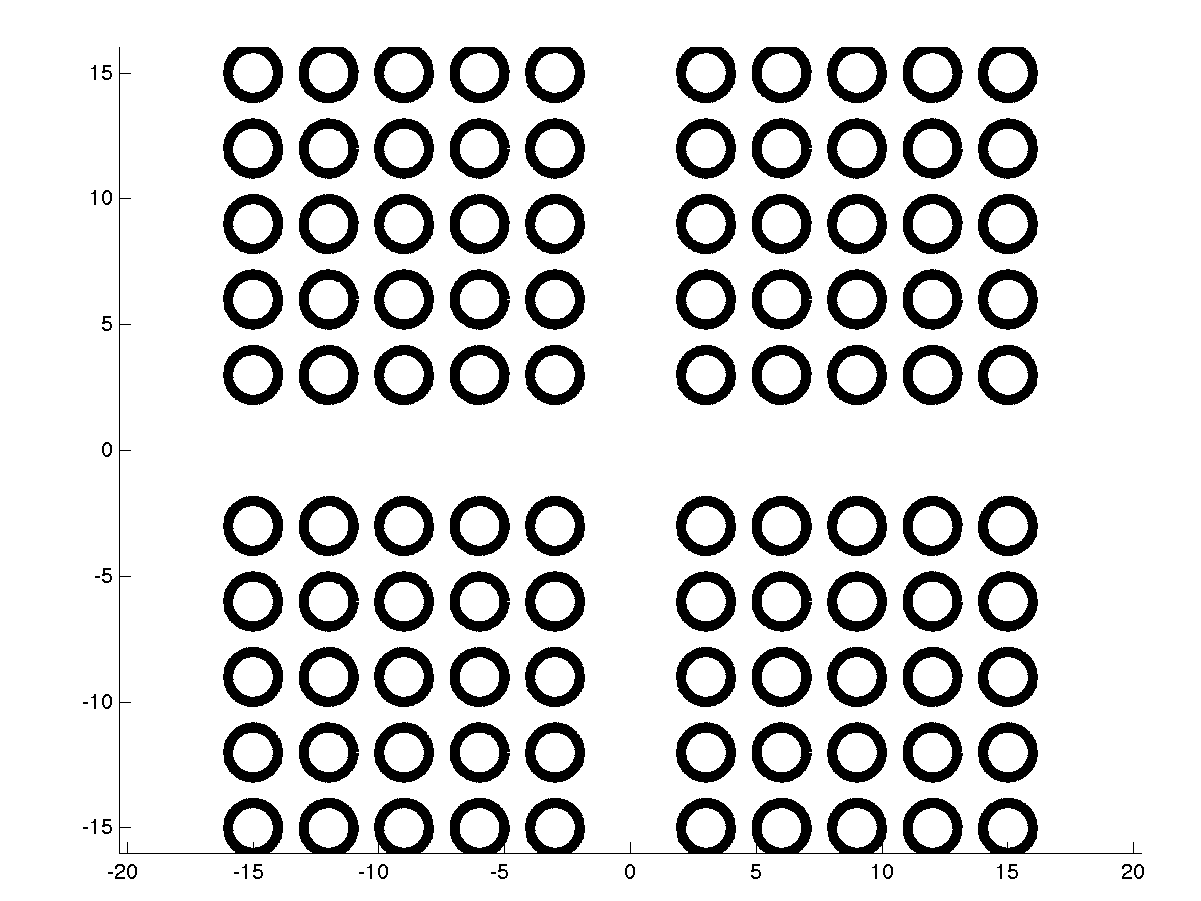
\includegraphics[width=0.45\textwidth]{./img/obstacles/removeDisks.png}}
 \draw (10pt,-75pt) node[below]{\footnotesize $x_{1}$} ;
 \draw (-92pt,10pt) node[below]{\footnotesize $x_{2}$} ;
\end{tikzpicture}
\caption{Periodic placement with a row and a column deleted.}
\label{fig:removeDisks}
\end{figure}



\subsection{Truncation of the Fourier series}
\label{secFun:FourierTruncation}

To help the user, the formula (\ref{eqEqInt:CFIEDapp}) has been computed in \mudiff. The values of $\Np$ are stored in a Matlab vector of size $[1\times\code{N\_scat}]$ called \code{M\_modes} in \mudiff. Computing \code{M\_modes} only involves the radii of the disks and the wavenumber \code{k}, which is assumed to be created by the user:
\begin{lstlisting}
M_modes = FourierTruncation(a, k);
\end{lstlisting}
The resulting vector is such that \code{M\_modes(p)}=$\Np$ where $\Np$ satisfies (\ref{eqEqInt:CFIEDapp}), with obviously a minimum value of $0$ (which consists of only one mode). If \code{k} is a vector (one wavenumber per obstacle), then \FourierTruncation compute formula (\ref{eqEqInt:CFIEDapp})  with \code{k(p)} as the wavenumber.

The following options are moreover availabe:
\begin{itemize}
\item \code{M\_modes = FourierTruncation(..., 'Min', MIN);}\\
To force a minimal value: \code{M\_modes(p)} is then either the min value between \code{MIN} and formula (\ref{eqEqInt:CFIEDapp}). 
\item\code{M\_modes = FourierTruncation(..., 'Tol', TOL);}
The tolerance, set by default to $10^{-10}$, is then set to \code{TOL}.
\end{itemize}

\subsection{Incident waves}

\subsubsection{Generalities}
\label{secFun:PlaneWave}
\label{secFun:DnPlaneWave}
\label{secFun:PointSource}
\label{secFun:DnPointSource}
\label{secFun:PlaneWavePrecond}
\label{secFun:DnPlaneWavePrecond}
\label{secFun:BlockPlaneWave}
\label{secFun:BlockDnPlaneWave}
\label{secFun:BlockPointSource}
\label{secFun:BlockDnPointSource}
\label{secFun:BlockPlaneWavePrecond}
\label{secFun:BlockDnPlaneWavePrecond}

Two different incident waves are available in the \mudiff toolbox: plane wave and point source wave. It should however be highlighted that the user can build his/her own incident wave. They are all located in \folder{PreProcessing/IncidentWave/}.

As explained in section \ref{secEqInt:SecondMembre}, a right-hand side $b$ is decomposed by blocks, each of these representing one obstacle: $b= (b_p)_{p=1,\ldots,\Nscat}$. A different condition can be applied on two different obstacles (\eg Dirichlet on $\Omega_1$ and Neumann on $\Omega_2$) or a different integral equation can be considered on it (\eg EFIE on $\Omega_1$ and MFIE on $\Omega_2$). To handle that, \mudiff builds each block separately thanks to \BlockIncidentWave, which computes the vector $b_p$. According to the input data, the function will build one of the available right-hand side described on table \ref{table:Uinc}.

On the other hand, the frontal function \IncidentWave computes the whole vector $b$. For every obstacle $p$, it calls \BlockIncidentWave and assembles the whole vector. 

In addition to this, for every incident waves, an interface function is available. They build the whole vector on only one pattern (trace of plane wave, normal derivative of point source wave, \ldots) but are very easy to use. They are located in the \folder{interface/} directory and their names are well chosen (see also table \ref{table:Uinc}, column \mudiff name): \PlaneWave, \PointSource, \DnPlaneWave,\ldots. Let us highlights that the help of the interface functions contains the mathematical description of the incident wave.

The two main functions, \BlockIncidentWave and \IncidentWave, are now detailed.

\subsubsection{\code{BlockIncidentWave}}
\label{secFun:BlockIncidentWave}

This functions computes the block vector of \textbf{the opposite of} the coefficients of an incident wave, either the trace of the normal derivative trace, on one of the obstacles, in the Fourier bases. Its syntax is
\begin{lstlisting}
Bp = BlockIncidentWave(Op, ap, Np, k, TypeOfWave, Param);
\end{lstlisting}
where \code{TypeOfWave} is a scalar value specifying the incident wave (see table \ref{table:Uinc}) and \code{Param} is the parameter of the wave: angle of direction, position of a point source, \ldots. The returned value \code{Bp} is a column vector of length $2\code{Np}+1$.
\begin{table}
\begin{tabular}{|c| c |c| p{9cm}| }
\hline Value & \mudiff name & Param & Type\\\hline
1 & \code{PlaneWave} & \code{beta\_inc} & Trace of a plane wave of angle of direction \code{beta\_inc}. A plane wave is defined by $e^{ik(\cos(\beta)x + \sin(\beta)y}$.\\\hline
2 & \code{DnPlaneWave} & \code{beta\_inc} & Normal derivative of a plane wave of angle of direction \code{beta\_inc}.\\\hline
3 & \code{PointSource} & \code{XS} & Trace of the wave emitted by a point source placed on \code{XS}. Such a wave is defined in \mudiff by $i/4\Hz(k\|\xx-\xx_s\|)$.\\\hline
4 & \code{DnPointSource} & \code{XS} & Normal derivative of the trace of the wave emitted by a point source placed on \code{XS}.\\\hline
5 & \code{PlaneWavePrecond} & \code{beta\_inc} & Same as \code{PlaneWave} but multiplied by the inverse diagonal of the single-layer diagonal block operator (see section \ref{} on single scattering preconditioner). \\\hline
6 & \code{DnPlaneWavePrecond} & \code{beta\_inc} & Same as \code{DnPlaneWave} but multiplied by the inverse diagonal of the double-layer diagonal block operator. \\\hline
\end{tabular}
\caption{Available right-hand sides}
\label{table:Uinc}
\end{table}

\subsubsection{\code{IncidentWave}}
\label{secFun:IncidentWave}

\begin{lstlisting}
B = IncidentWave(O, a, M_modes, k, TypeOfWave, Param)
\end{lstlisting}
The resulting vector \code{B} is of size $\sum_{p=1}^{\Nscat}(2\code{M\_modes}(p)+1)$. The value \code{Param} is the same as for \BlockIncidentWave whereas \code{TypeOfWave} is a vector of size $\Nscat$ where \code{TypeOfWave}(p) is the desired choice for the block $b_p$. In other word, the block $b_p$ will be built by calling \code{BlockIncidentWave(Op, ap, Np, k, TypeOfWave, Param);}. To simplify, if \code{TypeOfWave} is a scalar value, then it is considered as a vector of the same scalar value.

\paragraph{Example1:} building a vector associated to the trace of an incident plane wave of direction \code{beta\_inc} is done thanks to the following command (the ``$1$ argument'' refers to \code{PlaneWave}):
\begin{lstlisting}
B = IncidentWave(O, a, M_modes, k,  1, beta_inc);
\end{lstlisting}
or using the interface function
\begin{lstlisting}
B = PlaneWave(O, a, M_modes, k, beta_inc);
\end{lstlisting}
\paragraph{Example 2:} For two obstacles and a point source centered on $(1,2)$, if $b_1$ is the trace of the wave and $b_2$ is the normal derivative trace, then
\begin{lstlisting}
B = IncidentWave(O, a, M_modes, k,  [3;4],[1;2]);
\end{lstlisting}
In other words, this builds the vector (\code{[3,4]} can be translated as \code{PointSource, DnPointSource}):
$$
b = \left(\begin{array}{c}
-\uinc|_{\Gamma_1}\\
-\dn\uinc|_{\Gamma_2}\\
\end{array}\right),
$$
where $\uinc = \frac{i}{4}\Hz(k\|\xx-\xx_s\|)$, with $\xx_s = [1,2]$.
\begin{remark}
Remember that the resulting vector corresponds to the opposite of the trace or normal derivative trace!
\end{remark}


\section{Integral operators}
\label{sec:ResolutionMuDiff}

\subsection{Generalities}

The functions defining the integral operators are in the directory \folder{IntOperators/} which has the \folder{Dense/}
and \folder{Sparse/} subdirectories for the dense (matrix) and sparse (@function) representations of the four basic integral operators used in scattering,
\ie $\Lb$, $\Mb$, $\Nb$ and $\Db$, given in their infinite version by respectively (\ref{eq:InfL}), (\ref{eq:InfM}), (\ref{eq:InfN}) and (\ref{eq:InfD}). Preconditioned versions of the operators by their single scattering operators \cite{Thi14}. In fact and following Proposition \ref{prop:SingleScat}, only $\widehat{L}L$ (EFIE Dirichlet) and $\widehat{D}D$ (EFIE Neumann) are available, as they are the only one needed for the Dirichlet and Neumann problems. These operators have moreover an analytic expression of every of their coefficients (see equations (\ref{eq:LL}) and (\ref{eq:DD}), in the infinite matrices case).

Two different type of storage are available with the \mudiff toolbox: dense and sparse. The assembly of matrix is however similar for both cases (only a few differences). \mudiff is close to the mathematics for the assembly process, in the sense that the matrix $\Ab$ of an integral operator is built block by block ($\Abpq$). For both storage, two main functions exist: a ``block'' function (\BlockIntegralOperator and \SpBlockIntegralOperator) and a whole matrix function (\IntegralOperator and \SpIntegralOperator), which assembles every blocks into one matrix. This separation permits to the user to either build a ``simple'' matrix of one operator or to construct a more ``complex'' matrix where each block represents a different operator or a linear combination of them. Note also that, every operator has functions of interface (located in \folder{Dense/Interface} or \folder{Sparse/Interface} folders). For example \SingleLayer is the interface function of \IntegralOperator to build the single-layer operator, and \BlockSingleLayer the one of \BlockIntegralOperator. The same applies for the sparse storage with a prefix \code{Sp}:  \SpSingleLayer,  \SpBlockSingleLayer.


The dense storage should be preferred for solving small scale problem, when the memory and the CPU cost is not a problem, where the sparse storage must be used when the limits are reached. For the sparse storage, which is detailed later, the matrices are stored as vectors and the matrix-vector product is then fast. The drawback being however some instability, in particular when the truncation of the Fourier series is not done properly. The formula (\ref{eqEqInt:CFIEDapp}) seems to give a stable result though \cite{AntChnRam08}.



%Two different type of storage are provided with the \mudiff toolbox: dense and sparse. The dense storage the whole matrix in memory whereas the sparse version uses the special structure of the matrix of an integral operator to store it. The sparse storage in \mudiff and this user guide has nothing to deal with the sparse storage provided in \matlab such as \texttt{sparse} function. The dense storage is easier to use and works pretty well for small scale problems. It also presents the advantage of providing the whole matrix of the integral operator, which can be useful for spectrum analysis for example. On the other hand, for a large number of circular obstacles and/or for large frequency, the memory storage becomes too important and the sparse version must be used. One should be however careful: the sparse matrix-vector product, based on the cross-correlation (\texttt{xcorr} \matlab function), is very sensitive to the number of modes chosen in the truncation of the Fourier series. Indeed, if too many modes are kept, the matrix-vector product show to be unstable. The formula (\ref{eqEqInt:CFIEDapp}) seems to provide stability.
%
%To explain how the code works, let us take an example of one of the four boundary integral operator $L,M,N$ or $D$ being discretized as a generic matrix $\Ab = (\Abpq)_{1\leq p,q\leq \Nscat}$. Let us highlight that \mudiff can manage more complexe matrices, where two different blocks are not the discretization of the same operators or can even be a linear combination of operators. Nevertheless, if $\Ap$ is one of the four boundary integral operators, then as highlighted in previous chapter, $\Ab$ has the following structure, for $p,q=1,\ldots,\Nscat$ and $p\neq q$:
%\begin{itemize}
%\item $\Abpp$ is diagonal.
%\item $\Abpq$ is full and can be divided as $\Abpq = \AbpqL\Tbpq\AbpqR$ where $\AbpqL$ and $\AbpqR$ are diagonal and called respectively the left and right part, and $\Tbpq = (\Tbpqmn))$, with $\Tbpqmn = i\pi e^{??}H_0^{(1)}(k\bpq)$, is a Toeplitz matrix.
%\end{itemize}
%In the sparse version, diagonal submatrices $\Abpp,\AbpqL$ and $\AbpqR$  are stored as a vector of size respectively $2\Np+1$, $2\Np+1$ and $2\Nq+1$, and the Toeplitz matrices $\Tbpq$ are stored as vectors of size $2\Np+2\Nq-1$.
%
%This section is naturally divided in two part, the first being devoted to the dense storage and the second to the sparse version. The assembly, the storage and the usage of the matrices being significantly different.

\subsection{Available integral operators and numbering}
\label{seccode:IntOp}
\label{secFun:BlockSingleLayer}
\label{secFun:BlockDnSingleLayer}
\label{secFun:BlockDoubleLayer}
\label{secFun:BlockDnDoubleLayer}
\label{secFun:BlockPrecondDirichlet}
\label{secFun:BlockPrecondNeumann}
\label{secFun:BlockCalderonProjector}
\label{secFun:BlockIdentity}
\label{secFun:SingleLayer}
\label{secFun:DnSingleLayer}
\label{secFun:DoubleLayer}
\label{secFun:DnDoubleLayer}
\label{secFun:PrecondDirichlet}
\label{secFun:PrecondNeumann}
\label{secFun:CalderonProjector}
\label{secFun:Identity}

As for the incident wave, for every operator, there exists a function that build the whole operator for the multiple scattering problem, both for dense and sparse storage. The available operators are listed on table \ref{table:IntOp}, with their unique identifier (integer), their name in \mudiff (useful to get their interface functions) and their definition.

\begin{table}
\begin{center}\begin{tabular}{|c| c| c|c|}
\hline Int. Op. & Identifier & Function & Definition for $\xx\in\Gamma$\\\hline\hline
- & 0 & - & Zero operator (null matrix)\\\hline
$I$ & 1 & \tabcode{Identity} & Identity\\\hline
$L$ & 2 & \tabcode{SingleLayer} & $\dsp L\rho(\xx) = \int_{\Gamma} G(\xx,\yy) \rho(\yy)\dd\yy$\\[0.25cm]\hline
$M$ & 3 & \tabcode{DoubleLayer} & $\dsp M\lambda(\xx) = -\int_{\Gamma} \dny G(\xx,\yy) \lambda(\yy)\dd\yy$\\[0.25cm]\hline
$N$ & 4 & \tabcode{DnSingleLayer} & $\dsp N\rho(\xx) = \dnx\int_{\Gamma} G(\xx,\yy) \rho(\yy)\dd\yy$\\[0.25cm]\hline
$D$ & 5 & \tabcode{DnDoubleLayer} & $\dsp D\lambda(\xx) = -\dnx\int_{\Gamma} \dny G(\xx,\yy) \lambda(\yy)\dd\yy$\\[0.25cm]\hline
$\hat{L}L$ & 6 & \tabcode{PrecondDirichlet} & Single-Layer preconditioned by its diagonal\\[0.25cm]\hline
$\hat{D}D$& 7 & \tabcode{PrecondNeumann} & Dn Double-Layer preconditioned by its diagonal\\[0.25cm]\hline
\end{tabular}\end{center}
\caption{Available operators, their unique identifier, function name (interface) and the mathematical definition. The zero function does not have an interface function and the sparse version is obtained by prefixing by \code{Sp} (\SpSingleLayer, \SpDnDoubleLayer,\ldots). The block interface functions are also prefixed by ``\code{Block}'' (\SpBlockSingleLayer, \BlockSingleLayer,\ldots)}
\label{table:IntOp}
\end{table}


\subsection{Dense storage}
\subsubsection{Building a block $\Abpq$}
\label{secFun:BlockIntegralOperator}

A sub matrix block can be created with the function \BlockIntegralOperator:
\begin{lstlisting}
Apq = BlockIntegralOperator(Op, ap, Np, Oq, aq, Nq, k, TypeOfOperator, Weight);
\end{lstlisting}
The \code{Weight} argument is optional and set to $1$ by default. The quantity \code{TypeOfOperator} specifies the integral operator to compute, thanks to the numbering of Table \ref{table:IntOp}. If \code{TypeOfOperator} is a scalar (\eg $=2$) then the resulting matrix \code{Apq} is the submatrix of the associated operator (\eg $\Lbpq$). If \code{TypeOfOperator} is a row (\eg \code{[1,3]}) then the sum of the two operators is done (\eg $\Ibpq+\Mbpq$). Finally the \code{Weight} quantity, of the same size as \code{TypeOfOperator}, is the constant to multiply the block with. The block is hence:
$$
\Abpq = \sum_{\ell=1}^{N}\code{Weight}(\ell).\code{Operator}(\ell)
$$
where \code{Operator}$(\ell)$ is one of the integral operator.

\paragraph{Example 1:} Building the single-layer block $\Lbpq$:
\begin{lstlisting}
Apq = BlockIntegralOperator(Op, ap, Np, Oq, aq, Nq, k, 1);
\end{lstlisting}
\paragraph{Example 2:} Build the whole matrix $0.5\Ibpq + \Nbpq$, appearing in the MFIE (\ref{eq:MFIE}):
\begin{lstlisting}
Apq = BlockIntegralOperator(Op, ap, Np, Oq, aq, Nq, k, [1, 4], [0.5, 1]);
\end{lstlisting}
\paragraph{Example 3:} The sum of the four blocks: $0.5\Lbpq + 1.5\Mbpq + 2.5\Nbpq + 3.5\Dbpq$:
\begin{lstlisting}
Apq = BlockIntegralOperator(Op, ap, Np, Oq, aq, Nq, k, [2, 3, 4, 5], 
                         [0.5, 1.5, 2.5, 3.5]);
\end{lstlisting}


\subsubsection{Assemble the matrix $\Ab$}
\label{secFun:IntegralOperator}

Now that the construction of a block is well understood, building a matrix is very easy thanks to the frontal function
\begin{lstlisting}
A = IntegralOperator(O, a, M_modes, k, TypeOfOperator, Weight);
\end{lstlisting}
As for \BlockIntegralOperator, the quantity \code{Weight} is optional and set to $1$ by default. Roughly speaking, \IntegralOperator will loop on every obstacle $p$ and $q$ and launch the following command
\begin{lstlisting}
Apq = BlockIntegralOperator(O(:,p), a(p), M_modes(p), O(:,q), a(q), M_modes(q), 
                                                    k, Tpq, Wpq);
\end{lstlisting}
and places \code{Apq} in the right block of the whole matrix. The quantities \code{Tpq} and \code{Wpq} are given by \code{TypeOfOperator} and \code{Weight} such that (\code{Weight} is of the same size of \code{TypeOfOperator} and so \code{Wpq} follows the same rules as \code{Tpq}):
\begin{itemize}
\item If \code{TypeOfOperator} is a scalar then \code{Tpq} = \code{TypeOfOperator}. 
\item If \code{TypeOfOperator} is a row or a column vector then \code{Tpq} is an array given by \code{Tpq} = \code{TypeOfOperator}. 
\item If \code{TypeOfOperator} is a matrix then \code{Tpq} = \code{TypeOfOperator(p,q)}. 
\item If \code{TypeOfOperator} is a $3D-$array then \code{Tpq} is an array and is given by \code{Tpq(:)} = \code{TypeOfOperator(p,q,:)}. 
\end{itemize}
%
%For example, this matrix will give,
%$$
%\left(\begin{array}{c c}
%2& 3\\
%4&5
%\end{array}\right)
%\longrightarrow
%\left(\begin{array}{c c}
%L^{1,1}& M^{2,1}\\
%N^{1,2} & D^{2,2}
%\end{array}\right)
%$$


\paragraph{Example 1:} The single-layer potential $L$
\begin{lstlisting}
L = IntegralOperator(O, a, M_modes, k, 2);
\end{lstlisting}
\paragraph{Example 2:} The operator of the MFIE for a Dirichlet boundary condition (\ref{eq:MFIE}), $0.5I + N$:
\begin{lstlisting}
A_MFIE = IntegralOperator(O, a, M_modes, k, [1,4], [0.5,1]);
\end{lstlisting}
\paragraph{Example 3:} The following operator for two obstacles only
$$
\left(\begin{array}{c c}
0.5 I_{1,1}+ M_{1,1} & L_{1,2}\\
D_{2,1} & 0.5 I_{2,2}+N_{2,2}
\end{array}\right)
$$
can be computed using a $3D$ array and the null operator:
\begin{lstlisting}
TypeOfOp = zeros(2,2,2); Weight = zeros(2,2,2);
TypeOfOp(:, 1,1) = [1, 3]; Weight(:, 1,1) = [0.5, 1]; %block A_{1,1}
TypeOfOp(:, 1,2) = [2, 0]; Weight(:, 1,2) = [1, 0]; %block A_{1,2}
TypeOfOp(:, 2,1) = [5, 0]; Weight(:, 2,1) = [1, 0]; %block A_{2,1}
TypeOfOp(:, 2,2) = [1, 4]; Weight(:, 2,2) = [0.5, 1]; %block A_{2,2}
A = IntegralOperator(O, a, M_modes, k, TypeOfOp, Weight);
\end{lstlisting}
\paragraph{Example 4:} The Brakhage-Werner integral equation for a Dirichlet problem (\ref{eqEqInt:BW})
\begin{lstlisting}
k = 1;
beta_inc = pi;
eta = i/k;
Uinc = PlaneWave(O, a, M_modes, k, beta_inc);
A = IntegralOperator(O, a, M_modes, k, [1, 2, 3], [0.5, -eta_BW, -1]);
psi = A \ Uinc;
\end{lstlisting}

\subsection{Sparse storage}
\label{secFun:SpBlockSingleLayer}
\label{secFun:SpBlockDnSingleLayer}
\label{secFun:SpBlockDoubleLayer}
\label{secFun:SpBlockDnDoubleLayer}
\label{secFun:SpBlockPrecondDirichlet}
\label{secFun:SpBlockPrecondNeumann}
\label{secFun:SpBlockIdentity}
\label{secFun:SpSingleLayer}
\label{secFun:SpDnSingleLayer}
\label{secFun:SpDoubleLayer}
\label{secFun:SpDnDoubleLayer}
\label{secFun:SpPrecondDirichlet}
\label{secFun:SpPrecondNeumann}
\label{secFun:SpIdentity}

Storing the matrices in a sparse way leads to a significant reduction in memory storage and a faster matrix-vector product. The linear system must then however be solved using an iterative solver only, as the matrix is no more fully stored. Combining linearly the matrices is still possible but this is done during the matrix-vector product. Indeed, summing two matrices of two different integral operators is not guaranteed to keep the special structure. If the problem involves (at least) two different integral operators, they must hence be computed separately.

\subsubsection{Compact storage}

To explain how the matrix is stored using \mudiff sparse storage, let $\Ab$ be the matrix of one of the four integral operators $L,M,N$ or $D$. The matrix $\Ab$ has the following special structure (for $p,q=1,\ldots,M$ and $p\neq q$):
\begin{itemize}
\item $\Abpp$ is diagonal
\item $\Abpq$ is full and can be divided as $\Abpq = \AbpqL\Tbpq\AbpqR$ where $\AbpqL$ and $\AbpqR$ are diagonal and called respectively the left and right part, and $\Tbpq = (\Tbpqmn))$, with $\Tbpqmn = i\pi e^{i(n-m)\alpha_{pq}}H_{n-m}^{(1)}(k\bpq)$, is a Toeplitz matrix: $\Tbpqmn = \Tbpq_{m+1,n+1}$.
\end{itemize}

The idea is that the diagonal matrices can be stored as a vector containing the diagonal only. A matrix-vector product between a diagonal matrix and a vector is then simply a point-to-point multiplication. The Toeplitz matrix can also be stored in a compact form as a vector and the matrix-vector product is handled by a cross-correlation (based on FFT). 

The diagonals part are stored in the $3D$ arrays $\AbL$ and $\AbR$ (``L'' for left part and ``R'' for the right part). The left part, $\AbL$ also carries the diagonal part of the matrix:
$$
\AbL(:,p,q) = \begin{cases}
\diag(\Abpp) & \text{ if }p=q,\\
\diag(\AbpqL) & \text{ otherwise,}
\end{cases}\qquad
\AbR(:,p,q) = \begin{cases}
0 & \text{ if }p=q,\\
\diag(\AbpqR) & \text{ otherwise.}
\end{cases}
$$
The matrix $\Tbpq$, of size $(2\Np+1) \times (2\Nq+1)$ is then also compacted as a Toeplitz matrix has the following structure
$$
\Tbpq = \left(\begin{array}{c c c c c}
t_1 & t_2 & t_3 & \ldots & t_{(2\Nq+1)} \\
t_{(2\Nq+1)+1} & t_{1} & t_{2} & \ldots & t_{(2\Nq+1)-1}\\
t_{(2\Nq+1)+2} & t_{(2\Nq+1)+1} & t_{1} & \ldots & t_{(2\Nq+1)-2}\\
\vdots & \ddots & \ddots& \ddots& \vdots\\
%t_{(2\Nq+1)+(2\Np+1)-2} & t_{(2\Nq+1)+(2\Np+1)-3} & t_{(2\Nq+1)+(2\Np+1)-4} &   \ldots & t_{(2\Np+1)+1}\\
t_{(2\Nq+1)+(2\Np+1)-1} & t_{(2\Nq+1)+(2\Np+1)-2} & t_{(2\Nq+1)+(2\Np+1)-3} &   \ldots  & t_{(2\Nq+1)-(2\Np+1)+1}
\end{array}\right)
$$
Clearly, the root vector containing the first row and the first column is enough to rebuild the matrix. This root vector, called $\AbpqM$, is of size $(2\Np+1)+ (2\Nq+1)-1 = 2\Np +2\Nq+1$ and such that:
$$
\AbpqM = \left(\begin{array}{c}
t_{(2\Nq+1)+(2\Np+1)-1}\\
t_{(2\Nq+1)+(2\Np+1)-2}\\
\vdots\\
t_{(2\Nq+1)+2}\\
t_{(2\Nq+1)+1}\\
t_{1}\\
t_{2}\\
t_{3} \\
\vdots\\
t_{(2\Nq+1), 1}\\
\end{array}\right).
$$
Finally, all these root vectors are stored in the $3D$ array $\AbM$:
$$
\AbM(:,p,q) = \begin{cases}
0 & \text{ if }p=q,\\
\AbpqM & \text{ otherwise.}
\end{cases}
$$

The whole matrix $\Ab$ is thus stored in three different parts: $\AbL$, $\AbM$ and $\AbR$. From the computer point of view, as a $3D$ array has a fix size in each direction, the second and third dimension of the arrays are both of size \code{N\_scat} and the length in the first dimension is given by:
\begin{center}
\begin{tabular}{| l | l | l | l |}
\hline $3D$-array & \multicolumn{3}{c|}{Length in the dimension\ldots}\\\cline{2-4}
& $1$ & $2$ & $3$\\\hline
$\AbL$ & $\dsp \max_p(2\Np+1)$ & \tabcode{N\_scat}& \tabcode{N\_scat}\\[0.2cm]\hline
$\AbM$ & $\dsp \max_{p}\max_{q\neq p}\left[(2\Np+1)+(2\Nq+1)-1\right]$& \tabcode{N\_scat}& \tabcode{N\_scat}\\[0.2cm]\hline
$\AbR$ & $\dsp \max_p(2\Np+1)$& \tabcode{N\_scat}& \tabcode{N\_scat}\\[0.2cm]\hline
\end{tabular}\end{center}
With this constraint, the vector $\AbL(:,p,q)$ can be larger than $2\Np+1$ and thus $\AbpqL$ must be extracted: $\AbpqL = \AbL(1:2\Np+1, p, p)$. The same occurs for $\AbM$ and $\AbR$. 

Finally, these $3D$ arrays are merged into a cell \code{A}, representing the matrix $\Ab$, such that, using the Matlab notations:
$$
\code{A}\{1\} = \AbL,\qquad \code{A}\{2\} = \AbM,\qquad\code{A}\{3\} = \AbR.
$$

\subsubsection{Fast matrix-vector product}

The matrix vector product between $\Ab$ and a vector $X$ is divided in different smaller operations. Let us look at $Y=\Ab X$ and more particularly at the $p^{th}$ component
$$
Y_p = \sum_{q} \Abpq X_q.
$$
Using the previous notations, it can be rewritten as
$$
Y_p = \AbppL X_p + \sum_{q\neq p} \AbpqL (\AbpqM (\AbpqR X_q)).
$$
As $\AbppL$, $\AbpqL$ and $\AbpqR$ are all diagonal (and stored as a vector), these matrix-vector products are easy to compute. The only difficulty is located in $\AbpqM Z_q$ (where $Z_q=\AbpqR X_q$), but it can be achieved in a fast way. Indeed, the discrete cross correlation product (\code{xcorr}) between $\AbpqM$ and $Z_q$ gives
$$
\widetilde{W}_q = \code{xcorr}(Z_q, \overline{\AbpqM}),
$$
where the over bar denotes a complex conjugation. And the result $W_q$ is then extracted from $\widetilde{W}_q$ by
$$
W_q = \widetilde{W}_q(2\Nq+1:2\Nq+1+2\Np).
$$
The matrix vector product between $\Ab$ and $X$ is then done in a fast way (cross correlation is fast using Fourier).


\subsubsection{\mudiff: assemble the matrix}
\label{secFun:SpBlockIntegralOperator}
\label{secFun:SpIntegralOperator}

The assembly process is very similar to the dense one, the difference being the prefix \code{Sp}. The block function is then called by
\begin{lstlisting}
SpBlockIntegralOperator(Op, ap, Np, Oq, aq, Nq, Nmax, k, TypeOfOperator, Weight);
\end{lstlisting}
The function returns three vectors corresponding to $\AbpqL$, $\AbpqM$ and $\AbpqR$. The major difference here is that \textbf{no linear combination of operators can be done during the assembly process} for the sparse representation. The quantity \code{TypeOfOperator} cannot hence be a vector but only a scalar. On the other hand, the full assembly of a matrix can be done through
\begin{lstlisting}
A = SpIntegralOperator(O, a, M_modes, k, TypeOfOperator, Weight);
\end{lstlisting}
The result is a Matlab \code{cell} of three component, where each of them is a $3D-$array. The quantity \code{TypeOfOperator} can be a scalar or a matrix (not a $3D$ array nor a vector!). If \code{TypeOfOperator} is a matrix, then the block $\Abpq$ is assumed to be of type \code{TypeOfOperator(p,q)}. The linear combination of operators can still be done, but must be specified in the matrix-vector product (see below). Note that a function exists to add the (weighted-)identity to a sparse operator (see below).

\paragraph{Example 1:} Creation of \mudiff sparse matrix of the single-layer operator $L$
\begin{lstlisting}
L = SpIntegralOperator(O, a, M_modes, k, 2);
\end{lstlisting}
\code{L} is now a cell of $3$ components! Note that we can use the interface function
\begin{lstlisting}
L = SpSingleLayer(O, a, M_modes, k);
\end{lstlisting}
\paragraph{Example 2:} For two obstacles, building the following matrix 
$$
\left(\begin{array}{c c}
M_{1,1} & 0.5L_{1,2}\\
1.5D_{2,1} & 2.5N_{2,2}
\end{array}\right)
$$
can be done with the below commands
\begin{lstlisting}
TypeOfOp = zeros(2,2); Weight = zeros(2,2);
TypeOfOp(1,1) = [3]; Weight(1,1) = [1]; %block A_{1,1}
TypeOfOp(1,2) = [2,]; Weight(1,2) = [0.5]; %block A_{1,2}
TypeOfOp(2,1) = [5]; Weight(2,1) = [1.5]; %block A_{2,1}
TypeOfOp(2,2) = [4]; Weight(2,2) = [2.5]; %block A_{2,2}
A = SpIntegralOperator(O, a, M_modes, k, TypeOfOp, Weight);
\end{lstlisting}

\subsubsection{Assembly: adding the identity}
\label{secFun:SpAddIdentity}

It is possible to add the identity (multiplied by a constant) to a sparse operator:
\begin{lstlisting}
A = SpAddIdentity(A, alpha, M_modes);
\end{lstlisting}
which simply returns $A = A+\alpha I$.

\paragraph{Example 1:} If \code{L} is the sparse representation of the single-layer operator, then
\begin{lstlisting}
L = SpIntegralOperator(O, a, M_modes, k, 2);
alpha_L = SpAddIdentity(L, 0.5, M_modes);
\end{lstlisting}
will compute $0.5L$.

\subsubsection{\mudiff: sparse matrix-vector product}
\label{secFun:SpMatVec}
\label{secFun:SpSingleMatVec}

A matrix vector product $Y = \Ab X$ is done thanks to 
\begin{lstlisting}
Y = SpMatVec(X, M_modes, ListOfOperators, Weight);
\end{lstlisting}
where \code{Weight} is optional. \code{ListOfOperators} is a \textbf{Matlab cell} (not an array! Make use of $\{\cdot\}$ instead of $[\cdot]$) containing every sparse matrices that the user want to use. The linear combination of the operators is done at that time at each matrix-vector product.

\paragraph{Example 1:} Computing $Y = \Lb X$ is done as follows:
\begin{lstlisting}
SpL = SpIntegralOperator(O, a, M_modes, k, 2);
Y = SpMatVec(X, M_modes, SpL);
\end{lstlisting}
\paragraph{Example 2:} Calculating $Y =(0.5*I + N)X$, where $I$ is the identity (\textbf{Beware the $\{\cdot\}$ !}):
\begin{lstlisting}
SpI = SpIdentity(O, a, M_modes);
SpN = SpDnSingleLayer(O, a, M_modes, k);
Y = SpMatVec(X, M_modes, {SpI, SpN}, [0.5, 1]);
\end{lstlisting}
This could also be done using \SpAddIdentity function:
\begin{lstlisting}
SpN = SpDnSingleLayer(O, a, M_modes, k);
A = SpAddIdentity(SpN, 0.5, M_modes);
Y = SpMatVec(X, M_modes, A);
\end{lstlisting}

\subsubsection{Solving a linear system}

Now that the matrices and the right hand side have been assembled, the sparse linear system can solved iteratively. Using for example the GMRES solver \cite{SaaSch86}, the syntax to solve\ldots
\paragraph{Example 1: The EFIE (\ref{eq:EFIE}):} $L\rho = -\uinc|_{\Gamma}$, would be
\begin{lstlisting}
SpL = SpSingleLayer(O, a, M_modes, k);
Uinc = PlaneWave(O, a, M_modes, k, beta_inc);
rho = gmres(@(X)SpMatVec(X, M_modes, SpL), Uinc);
\end{lstlisting}
\paragraph{Example 2: The MFIE (\ref{eq:MFIE}):} $(I/2+N)\rho = -\dn\uinc|_{\Gamma}$:
\begin{lstlisting}
SpN = SpDnSingleLayer(O, a, M_modes, k);
SpI = SpIdentity(O, a, M_modes);
DnUinc = DnPlaneWave(O, a, M_modes, k, beta_inc);
rho = gmres(@(X)SpMatVec(X, M_modes, {SpI, SpN}, [0.5, 1]), DnUinc);
\end{lstlisting}
or using the \SpAddIdentity function
\begin{lstlisting}
SpAMFIE = SpDnSingleLayer(O, a, M_modes, k);
SpAMFIE = SpAddIdentity(SpAMFIE, 0.5, M_modes);
DnUinc = DnPlaneWave(O, a, M_modes, k, beta_inc);
rho = gmres(@(X)SpMatVec(X, M_modes, SpAMFIE), DnUinc);
\end{lstlisting}
\paragraph{Example 3: The Brakhage-Werner integral equation} for a Dirichlet problem (\ref{eqEqInt:BW})
\begin{lstlisting}
k = 1;
beta_inc = pi;
eta = i/k;
Uinc = PlaneWave(O, a, M_modes, k, beta_inc);
SpA = SpIntegralOperator(O, a, M_modes, k, [1, 2, 3], [0.5, -eta_BW, -1]);
psi = gmres(@(X)SpMatVec(X, M_modes, SpA), Uinc);
\end{lstlisting}


\section{Post-Processing}
\label{sec:PostProcessing}

Now that the system has been solved, the next step is to display some results. The \mudiff toolbox proposes some post-processing features such as computing the far-field (fast) or the near-field of the wave on a grid (Matlab \code{meshgrid}) or on some points only. In addition, other features are available such as drawing the disks on figures or the incident field. Both the near- and far-field computations can be done for a linear combination of a single- and double-layer potentials $\Lop\rho + \Mop\lambda$, only one of them (\eg $\Lop\rho$) or with the same density $(\Lop+\Mop)\psi$, with a single command line. Every post-processing functions are located in the \folder{PostProcessing/} directory.

\subsubsection{Far field}
\label{secFun:FarField}
\label{secFun:FarFieldSingleLayer}
\label{secFun:FarFieldDoublleLayer}

The far field of the single- and double-layer potentials
$$
\sum_{p=1}^{\Nscat}\eta_p\Lop_p\rho_p + \gamma_p\Mop_p\lambda_p,
$$
is given by equation (\ref{eq:FFFourier}). The \FarField function does the job properly:
\begin{lstlisting}
F = FarField(O, a, M_modes, k, theta, Density, Weight);
\end{lstlisting}
where the parameters are:
\begin{itemize}
\item \code{theta} is the vector of receiving angles (in rad.)
\item \code{Density} is either $\rho$, $\lambda$ or both. If \code{Density} is a column vector then \code{Density(:,2)} = \code{Density(:,1)} and only one density is used both for the single- and the double-layer potentials contribution. If \code{Density} has $2$ columns, then \code{Density(:,1)} is considered to be the single-layer density and \code{Density(:,2)} the double-layer density.
\item \code{Weight} is the weights to apply to the $\Nscat$ volumic integral operators ($\eta_p$ and $\gamma_p$). The quantity \code{Weight} is of size either $[1\times2]$ or $[1\times\Nscat]$. The first column of \code{Weight} is applied to the single-layer potentials and the second to the double-layer potentials: \code{Weight(p,1)}=$\eta_p$ and \code{Weight(p,2)}=$\gamma_p$. If \code{Weight} is a row of length $2$ then \code{Weight(1)}=$\eta_p$ and \code{Weight(2)}=$\gamma_p$ for all $p$ (the coefficient are the same for every obstacles).
\end{itemize}
With these notations, the far field computed is the far field of:
$$
\sum_{p=1}^{\code{N\_scat}}\code{Weight(p, 1)}\Lop\code{Density(:,1)} + \code{Weight(p,2)}\Mop\code{Density(:,2)}.
$$
\paragraph{Example 1:}  EFIE for the Dirichlet problem (\ref{eq:EFIE}, where the scattered field $u$ reads as $u = \Lop\rho$, its far field is then computed by
\begin{lstlisting}
F = FarField(O, a, M_modes, k, theta, rho, [1,0]);
\end{lstlisting}
\paragraph{Example 2:} for the Brackage-Werner integral equation for the Dirichlet problem (\ref{eqEqInt:BW}),  the scattered field $u$ reads as $u = (-\eta\Lop-\Mop)\psi$, and its far field is computed by
\begin{lstlisting}
eta = i/k;
F = FarField(O, a, M_modes, k, theta, psi, [-eta,-1]);
\end{lstlisting}
\paragraph{Example 3:} $\rho$ and $\lambda$ are both computed and the user needs to compute for example
$$
\sum_{p=1}^{\Nscat} p\Lop_p\rho_p - p\Mop_p\lambda_p,
$$
then (s)he can do it with: 
\begin{lstlisting}
F = FarField(O, a, M_modes, k, theta, [rho, lambda], [[1:p].', -[1:p].']);
\end{lstlisting}

\begin{remark}
The \FarField function is also interfaced with ready-to-use function: \FarFieldSingleLayer and \FarFieldDoubleLayer. These are located in the \folder{PostProcessing/FarField/Interface} directory.
\end{remark}

\subsubsection{Radar Cross Section (RCS)}
\label{secFun:RCS}
\label{secFun:RCSSingleLayer}
\label{secFun:RCSDoubleLayer}
\label{secFun:FarFieldtoRCS}

The radar cross section of a far field can be computed either from the far field with \FarFieldtoRCS or directly from the density with \RCS. In \mudiff, the radar cross section $\sigma$ is obtained by ($F$ being the far field)
$$
\sigma = 10\log_{10}(2\pi|F|^2).
$$
The computation is then done by typing:
\begin{lstlisting}
R = FarField_to_RCS(F);
\end{lstlisting}
where \code{F} has been computed by the \FarField function. Otherwise, the RSC can be computed directly from the densities by
\begin{lstlisting}
R = RCS(O, a, M_modes, k, theta, Density, Weight);
\end{lstlisting}
where the arguments are exactly the same as for the far field. In fact, \RCS first calls \FarField and then \FarFieldtoRCS.

\begin{remark}
The \RCS function is also interfaced with the two following ready-to-use functions \RCSSingleLayer and \RCSDoubleLayer. Both of them are located in the \folder{PostProcessing/FarField/Interface} directory.
\end{remark}


\subsubsection{Near field: outside and inside the obstacles}
\label{secFun:ExternalPotential}
\label{secFun:InternalPotential}
\label{secFun:ExternalSingleLayerPotential}
\label{secFun:ExternalDoubleLayerPotential}
\label{secFun:InternalSingleLayerPotential}
\label{secFun:InternalDoubleLayerPotential}
\label{secFun:GetPotentialOptions}
\label{secFun:BlockPotential}

The near field of a potential is given by equations (\ref{eqEqInt:Lphimpt}) and (\ref{eqEqInt:Mphimpt}) outside the obstacles and by (\ref{eqEqInt:LphimptINT}) and (\ref{eqEqInt:MphimptINT}) inside. In the same way, \mudiff separates the outside and the inside computation. 

First is explained how to compute the field outside the obstacles. The user only needs to create a mesh using \eg \code{meshgrid} and launch \ExternalPotential, which syntax is
\begin{lstlisting}
U = ExternalPotential(X, Y, O, a, M_modes, k, Density, Weight, OPTIONS);
\end{lstlisting}
The resulting matrix \code{U} has $0$ value inside the obstacle. By default, the computation is not done on the boundary of the obstacles (this can be changed thanks to the options). The arguments are:
\begin{itemize}
\item The arguments \code{Density} and \code{Weight} are exactly the same as for \FarField,
\item The quantities \code{X} and \code{Y} are the grid and they come from the Matlab \code{meshgrid} function
\item The OPTIONS must be chosen from the options of the potential, see below (after the internal potential).
\end{itemize}

Second, the computation inside the obstacle $\Omega_p$. For the inside field, the only contribution is assumed to be of the form 
$$
\Lop_p\rho_p + \Mop_p\lambda_p
$$
In other words, the contributions of the other obstacles are not taken into account. In the same way as for the external potential, the computation is done in \mudiff with:
\begin{lstlisting}
U = InternalPotential(X, Y, O, a, M_modes, k, Density, Weight, OPTIONS);
\end{lstlisting}
where \code{U} has zero value outside the obstacles and by default, also on the boundaries. The arguments are exactly the same as \ExternalPotential.

Finally, the common options for \ExternalPotential and \InternalPotential are described below. For the sake of clarity, the examples are shown with only \ExternalPotential even if they work also for \InternalPotential:
\begin{itemize}
\item \code{ExternalPotential(..., 'Verbosity', VERBOSITY)}\\
\code{VERBOSITY} is a scalar, which when set to 0, stop displaying message (default = 1)
\item \code{ExternalPotential(..., 'OnBoundary', ONBOUNDARY)}\\
if \code{ONBOUNDARY} is set to $1$ then the boundary is also covered (beware of the jump relation\ldots) (default = 0)
\end{itemize}

\paragraph{Example 1: }compute the single-layer potential $u=\Lop\rho$ on a grid:
\begin{lstlisting}
XX = [-10:0.1:10];
YY = [-10:0.1:10];
[X,Y] = meshgrid(XX,YY);
U = ExternalPotential(X, Y, O, a M_modes, k, rho, [1,0]);
\end{lstlisting}

\paragraph{Example 2: } consider two obstacles and compute $\Lop_1\rho_1 + 0.5\Lop_2\rho_2 + 1.5\Mop_1\lambda_1 -1.5\Mop_2\lambda_2$  inside the obstacle, where the densities are assumed to be computed:
\begin{lstlisting}
XX = [-10:0.1:10];
YY = [-10:0.1:10];
[X,Y] = meshgrid(XX,YY);
U = InternalPotential(X, Y, O, a M_modes, k, [rho, lambda], [1, 1.5 ; 0.5, -1.5]);
\end{lstlisting}

\begin{remark}
The near field functions \ExternalPotential and \InternalPotential are also interfaced by: \ExternalSingleLayerPotential, \InternalSingleLayerPotential, for the single-layer and by \ExternalDoubleLayerPotential and \InternalDoubleLayerPotential for the double layer potential. These four ready-to-use functions are located in the folder \folder{PostProcessing/NearField/Interface}.
\end{remark}

\subsubsection{Incident wave}
\label{secFun:IncidentWaveOnGrid}

The incident waves can be also computed on a grid using 
\begin{lstlisting}
Uinc = IncidentWaveOnGrid(X, Y, k, TypeOfWave, Param);
\end{lstlisting}
where, as for the \IncidentWave function from the PreProcessing part (see \S\ref{secFun:IncidentWave}) :
\begin{itemize}
\item \code{X} and \code{Y} ares matrices coming from the \code{meshgrid} Matlab function
\item \code{Param} is either the angle of direction for a plane wave (scalar) or the location of a point source ($[2\times1]$ vector)
\item \code{TypeOfWave} is either a \code{char} or a scalar value 
\end{itemize}
\paragraph{Example:} computation of a plane wave of angle of direction \code{beta\_inc}=$\pi$:
\begin{lstlisting}
beta_inc = pi;
XX = [-10:0.1:10];
YY = [-10:0.1:10];
[X,Y] = meshgrid(XX,YY);
Uinc = IncidentWaveOnGrid(X, Y, k, 'PlaneWave', beta_inc);
\end{lstlisting}
The last line could also be (switch \code{'PlaneWave'} with its identifier $1$):
\begin{lstlisting}
Uinc = IncidentWaveOnGrid(X, Y, k, 1, beta_inc);
\end{lstlisting}

 
\subsubsection{Geometry: drawing the obstacles and creating mask matrices}
\label{secFun:PlotCircles}
\label{secFun:MaskMatrixObstacles}
\label{secFun:BoundaryOfObstacles}


The \mudiff toolbox also proposes some functions for the post processing of obstacles. 
\paragraph{Drawing the disks with \PlotCircles}\mbox{}
\begin{lstlisting}
PlotCircles(O, a, fig_index, OPTIONS);
\end{lstlisting}
where \code{fig\_index} is the Figure handle and the OPTIONS are
\begin{itemize}
\item \code{PlotCirclesOnFigure(..., 'Color', COLOR)}: apply the \code{COLOR} color to lines (same as the plot function)
\item \code{PlotCirclesOnFigure(..., 'LineWidth', LINEWIDTH)}: set the line width to \code{LINEWIDTH} (same as the plot function)
\item \code{PlotCirclesOnFigure(..., 'zdata', ZDATA)}: set the zdata of the figure to \code{ZDATA} (same as the plot function)
\end{itemize}
Remark that, when drawing disks on a figure containing some values, do not forget to set the zdata to the max value! Examples: 
\begin{lstlisting}
figure(1);
surf(X,Y,U);
PlotCirclesOnFigure(O, a, 1, 'zdata', max(max(U)));
\end{lstlisting}

\paragraph{Getting a mask matrix,} which is a matrix $S$ such that, if $X$ and $Y$ are obtained by \code{meshgrid}:
$$
S(i,j) = \begin{cases}
0 & \text{ if } (X(i,j),Y(i,j)) \text{ is outside the obstacles,}\\
p & \text{ if } (X(i,j),Y(i,j)) \in\Omega_p,\\
p+0.5 & \text{ if } (X(i,j),Y(i,j)) \in\Gamma_p.\\
\end{cases}
$$
This kind of matrix is handy when plotting the potentials and is actually used by the two functions \ExternalPotential and \InternalPotential. The function \MaskMatrixObstacles which provides the matrix $M$ has the following syntax
\begin{lstlisting}
S = MaskMatrixObstacles(X, Y, O, a);
\end{lstlisting}

\paragraph{Extract the boundary points.} In the same way as the \MaskMatrixObstacles function, \BoundaryOfObstacles leads to a matrix $G$ where
$$
G(i,j) = \begin{cases}
0 & \text{ if } (X(i,j),Y(i,j)) \text{ is outside the obstacles,}\\
0 & \text{ if } (X(i,j),Y(i,j)) \in\Omega_p,\\
p & \text{ if } (X(i,j),Y(i,j)) \in\Gamma_p.\\
\end{cases}
$$
Similarly, $G$ is computed by
\begin{lstlisting}
G = BoundaryOfObstacles(X, Y, O, a);
\end{lstlisting}

\section{Full Examples}

Some examples are available in the \folder{Examples/} directory and especially in \folder{Examples/Benchmark}, where each files is independent and solve a different problem (Dirichlet, Neumann or Penetrable). They should also be launched as a tested, to verify that \mudiff is correctly installed and working properly. Next chapter also present some classical examples.











